% https://www.overleaf.com/learn/latex/Beamer#Using_a_colorthemev

% Inbuilt themes in beamer
\documentclass[8pt, aspectratio=169]{beamer}

\input{../template/macros/macros_general.tex}
\input{../template/macros/macros_math.tex}
\input{../template/symbols/symbols_NN.tex}
\input{../template/symbols/symbols_robot.tex}

% ~~~~~~~~~~~~~~~~~~~~~~~~~~~~~~~~~~~~~~~~~~~~~~~~~~~~~~~~~~~~~~~~~~~~~~~~~~~~~~
% Block options: Default, Alert, Example
% ~~~~~~~~~~~~~~~~~~~~~~~~~~~~~~~~~~~~~~~~~~~~~~~


% % Theme choice:
% \usetheme{Antibes}
% % \usecolortheme{beaver}
%~~~~~~~~~~~~~~~~~~~~~~~~~~~~~~~~~~~~~~~~~~~~~~~~~~~~~~~~~~~~~~~~~~~~~~~~~~~~~~
% Use roboto Font (recommended)
% \usepackage[sfdefault]{roboto}
\usepackage[utf8]{inputenc}
\usepackage[T1]{fontenc}
%~~~~~~~~~~~~~~~~~~~~~~~~~~~~~~~~~~~~~~~~~~~~~~~~~~~~~~~~~~~~~~~~~~~~~~~~~~~~~~

%~~~~~~~~~~~~~~~~~~~~~~~~~~~~~~~~~~~~~~~~~~~~~~~~~~~~~~~~~~~~~~~~~~~~~~~~~~~~~~
% Define where theme files are located. ('/styles')
\usepackage{styles/fluxmacros}
\usefolder{styles}
% Use Flux theme v0.1 beta
% Available style: asphalt, blue, red, green, gray 
\usetheme[style=blue]{flux}
%~~~~~~~~~~~~~~~~~~~~~~~~~~~~~~~~~~~~~~~~~~~~~~~~~~~~~~~~~~~~~~~~~~~~~~~~~~~~~~

%~~~~~~~~~~~~~~~~~~~~~~~~~~~~~~~~~~~~~~~~~~~~~~~~~~~~~~~~~~~~~~~~~~~~~~~~~~~~~~
% Extra packages for the demo:
\usepackage{booktabs}
\usepackage{colortbl}
\usepackage{ragged2e}
\usepackage{schemabloc}
%~~~~~~~~~~~~~~~~~~~~~~~~~~~~~~~~~~~~~~~~~~~~~~~~~~~~~~~~~~~~~~~~~~~~~~~~~~~~~~
\usepackage{calc}

\usepackage{svg}
\usepackage{media9}             %pdflatex, latex+dvips+ps2pdf, xelatex
\usepackage{multimedia}
\usepackage{animate}

% Title page details: 
\title{
    Imposing a Weight Norm Constraint for Neuro–Adaptive Control 
} 
\subtitle{
    \textit{IEEE European Control Conference (ECC) 2025}\\
}
\author{Myeongseok Ryu\inst{1}, Jiyun Kim\inst{2}, and Kyunghwan Choi\inst{1}}
\date{\today}
% \institute[short]{\inst{1} First \samelineand \inst{2} Second \samelineand \inst{3} Third}
\newcommand{\samelineand}{\\}
\institute{%
    \begin{minipage}[c]{\linewidth}
        \centering
        \inst{1}%
        Department of Mechanical and Robotics Engineering\\
        Gwangju Institute of Science and Technology
        \and
        \inst{2}%
        AI Graduate School\\
        Gwangju Institute of Science and Technology
  \end{minipage}
}
% make institute font size smaller
\setbeamerfont{institute}{size=\normalsize}

\logo{
  \vspace{-.7cm}%
  
\includegraphics[height=0.3cm]{assets/MIC_Lab_logo.jpg}
  
\includegraphics[height=0.3cm]{assets/kaist_logo.png}
  \hspace{.6cm}%
  }

\AtBeginSection[]{%
  \frame<beamer>{ 
    \frametitle{Outline}   
    \tableofcontents[currentsection] 
  }
}

% \AtBeginSubsection[]{%
%   \begin{frame}
%   \vfill
%   \centering
%     \insertsectionhead
%     \\
%     \large\textbf{\insertsubsectionhead}
%   \vfill
%   \end{frame}
% }

\titlegraphic{logo_KAIST.png}

\begin{document}

% Title page frame
% \begin{frame}
\titlepage 
% \end{frame}

% Outline frame
\begin{frame}{Outline}
    \tableofcontents
\end{frame}

% Lists frame
\section{Background and Contributions}

\subsection{Introduction to Neuro–Adaptive Control}

\begin{frame}{\insertsubsectionhead}{What is Neuro–Adaptive Control?}

  \textbf{Neuro–Adaptive Control}
  \small{
    \begin{itemize}
      \item \textbf{Neuro–adaptive control} (NAC) is a control strategy that combines \textbf{neural networks (NNs)} with \textbf{adaptive control techniques} \cite{Farrell:2006aa}.
      \item It is used to handle \textbf{uncertainties} and \textbf{nonlinearity} in dynamic systems. 
    \end{itemize}
  }

  \begin{figure}
    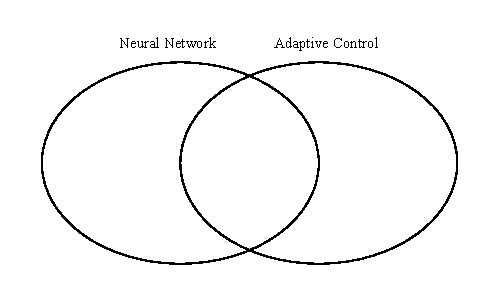
\includegraphics[width=0.55\textwidth]{figures/NAC.drawio.pdf}
  \end{figure}

\end{frame} 


\begin{frame}{\insertsubsectionhead}{What is Neuro–Adaptive Control?}

  \textbf{Advantages of Neuro-Adaptive Control}
  \small{
    \begin{itemize}
      \item \textbf{Adaptability}: NAC adapts to changing environments and system dynamics.
      \item \textbf{Stability Guarantee}: The closed-loop stability is ensured using \textbf{Lyapunov stability theory}.
      \item \textbf{Online Learning Capability}: NAC adapts in \textbf{real-time} to new data with stability guarantees.
      \item \textbf{Robustness}: NAC handles \textbf{uncertainties and disturbances} effectively with adaptive control techniques.
    \end{itemize}
  }
  
\end{frame}

\begin{frame}{\insertsubsectionhead}{Existing Challenges in NAC}
  
  \textbf{Challenges}
  \small{
    \begin{itemize}
      \item \textbf{Optimality}: In general, the adaptation laws are driven with respect to the tracking error, which may not guarantee optimal performance.
      \item \textbf{Unpredictable Amplitude of NN Weights}: 
        \begin{itemize}
          \item NN weights may diverge, leading to instability.
          \item This can result in unpredictable behavior of the controller.
        \end{itemize}
      \item \textbf{Parameter Dependency}: 
    \end{itemize}
  }

  \begin{figure}
    
\includegraphics[width=0.25\textwidth]{figures/KAIST-hi.png}
  \end{figure}

\end{frame}

\subsection{Literature Review}

\begin{frame}{\insertsubsectionhead}
  
  In general, the NN outputs are bounded by limiting the maximum amplitude of the NN weights.

  \begin{enumerate}
    \begin{columns}[T,onlytextwidth]
        \column{0.49\textwidth}
          \item \textbf{Projection Operator}

          \begin{itemize}
            \item Cats 
            \item Dogs 
            \item Birds
          \end{itemize}

        \column{0.49\textwidth}
          \begin{figure}
            
\includegraphics[width=0.4\textwidth]{figures/KAIST-hi.png}
          \end{figure}
      \end{columns}

      \begin{columns}[T,onlytextwidth]
        \column{0.49\textwidth}
          \item \textbf{$\epsilon$-modification, and $\sigma$-modification}

          \begin{itemize}
            \item Cats 
            \item Dogs 
            \item Birds
          \end{itemize}

        \column{0.49\textwidth}
          \begin{figure}
            
\includegraphics[width=0.4\textwidth]{figures/KAIST-hi.png}
          \end{figure}
      \end{columns}
  \end{enumerate}
\end{frame}

\subsection{Research Objectives}

\begin{frame}{\insertsubsectionhead}

  \textbf{Objective 1: Optimality}
  \begin{itemize}
    \item Formulate a constrained optimization problem to minimize the tracking error.
    \item Guarantee the stability of the system and the NN weights.
  \end{itemize}

  \textbf{Objective 2: Stability}
  \begin{itemize}
    \item Derive an adaptation law that guarantees the stability of the system.
    \item Ensure that the NN weights remain bounded during operation.
  \end{itemize}

  \textbf{Objective 3: Boundedness of }
  \begin{itemize}
    \item Ensure the controller is robust to uncertainties and disturbances.
    \item Validate the proposed method through numerical simulations.
  \end{itemize}

\end{frame}

\section{Proposed Method}

\subsection{Problem Formulation}

\begin{frame}{\insertsubsectionhead}{Original Control Problem}
  \textbf{Objectives}:
  \begin{itemize}
    \item Minimize the tracking error by adapting the NN weights $\estwth$.
    \item Guarantee the stability of the system and the NN weights $\estwth$.
  \end{itemize}
  
  \begin{figure}
    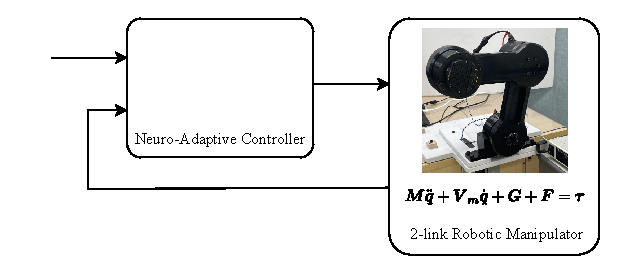
\includegraphics[width=0.5\textwidth]{figures/problem.drawio.pdf}
    % \includesvg{figures/problem.drawio}
    \caption{Architecture of the constrained optimization-based neuro-adaptive controller (CONAC).}
  \end{figure}

  \let\thefootnote\relax\footnote{
    \textit{Notations}: 
      $\mm{M}$: Inertia matrix, $\mm{C}$: Coriolis matrix, $\mm{G}$: Gravity vector, $\mv{\tau}$: Control input, $\mv{q}$: Joint position, $\estwth$: Estimated NN weights.
      }

\end{frame}

\begin{frame}{\insertsubsectionhead}{Equvalent Constrained Optimization Problem}

\end{frame}

\begin{frame}{\insertsubsectionhead}{Inequality Constraint for Weight Boundedness}

\end{frame}

\subsection{Adaptation Law Derivation}

\begin{frame}{\insertsubsectionhead}{Steepest Descent Method}


\end{frame}
\subsection{Stability Analysis}

\begin{frame}{\insertsubsectionhead}{Lyapunov Stability Analysis}


\end{frame}

\section{Numerical Validation}

\subsection{Simulation Setup}
\begin{frame}{\insertsubsectionhead}{2-Link Robotic Manipulator}
    
\end{frame}

\subsection{Simulation Results}

\begin{frame}{Representative Simulation Results}

  % % \movie[width=3cm,height=2cm,poster]{}{overall.mp4}
  % \begin{figure}
  %   \centering
  %   \href{https://youtu.be/U5uDbJQkGY8}{
  %     
\includegraphics[width=.1\textwidth]{figures/KAIST-hi.png}
  %   }
  % \end{figure}

  % \animategraphics[loop,width=4cm]{gifs/overall-}
  \animategraphics[loop,width=4cm]{10}{gifs/overall-}{0}{10}


\end{frame}

\begin{frame}{Box-and-Whisker Plots}
  
  \begin{columns}
    \column{0.5\textwidth}
      \begin{figure}
        \includegraphics[width=\textwidth]{figures/BoxWhisker.drawio.png}
        \caption{Parameter dependencies of the proposed method.}
      \end{figure}

    \column{0.5\textwidth}
      \begin{table}
        \caption{Largest cities in the world (source: Wikipedia)}
        \begin{tabular}{@{} lr @{}}
          \toprule
          City & Population\\
          \midrule
          Mexico City & 20,116,842\\
          Shanghai & 19,210,000\\
          Peking & 15,796,450\\
          Istanbul & 14,160,467\\
          \bottomrule
        \end{tabular}
    \end{table}
    
  \end{columns}

\end{frame}

\begin{frame}{Parameter Dependencies}

  \begin{columns}

    \column{0.33\textwidth}
      \begin{figure}      
        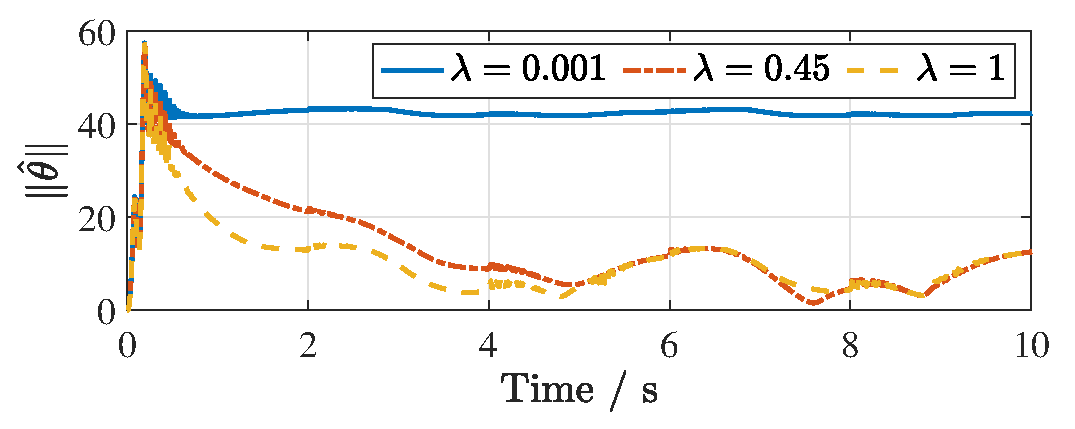
\includegraphics[width=0.99\textwidth]{figures/ECC/fig9.eps}
        \caption{Weight norms of NAC-L2}
      \end{figure}
      
    \column{0.33\textwidth}

      \begin{figure}
        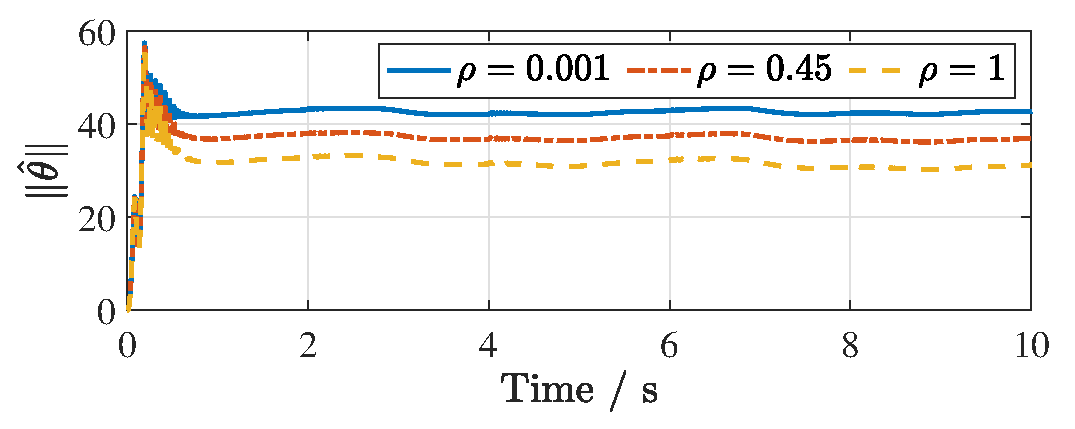
\includegraphics[width=0.99\textwidth]{figures/ECC/fig10.eps}
        \caption{Weight norms of NAC-eMod}
      \end{figure}

    \column{0.33\textwidth}

      \begin{figure}
        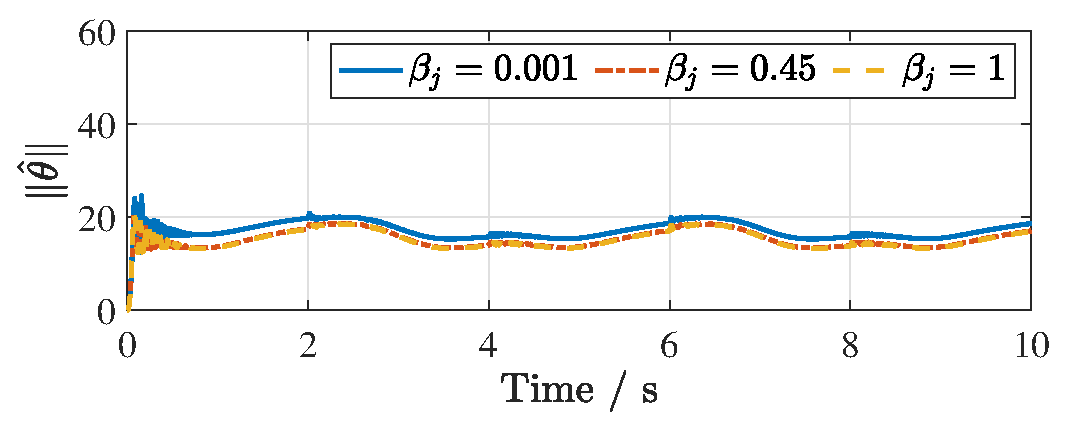
\includegraphics[width=0.99\textwidth]{figures/ECC/fig8.eps}
        \caption{Weight norms of NAC-CO}
      \end{figure}
    
  \end{columns}

  The weight norms of the proposed method (NAC-CO) are bounded, while ...

\end{frame}

\begin{frame}{Parameter Dependencies}

  \begin{columns}

    \column{0.33\textwidth}
      \begin{figure}      
        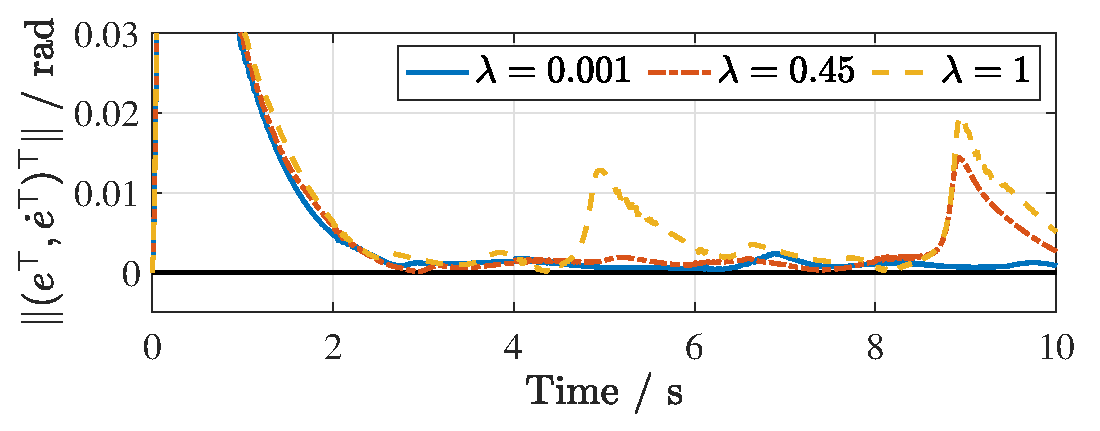
\includegraphics[width=0.99\textwidth]{figures/ECC/fig6.eps}
        \caption{Tracking error of NAC-L2}
      \end{figure}
      
    \column{0.33\textwidth}

      \begin{figure}
        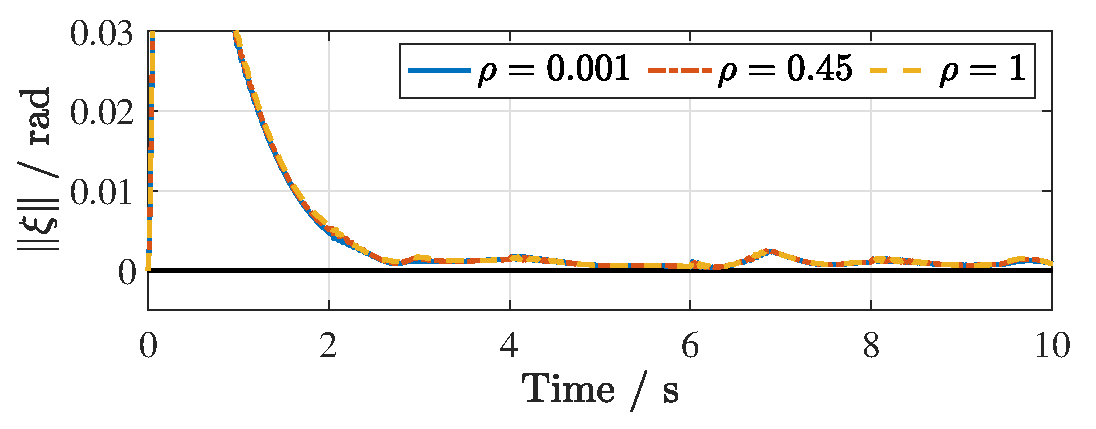
\includegraphics[width=0.99\textwidth]{figures/ECC/fig7.eps}
        \caption{Tracking error of NAC-eMod}
      \end{figure}

    \column{0.33\textwidth}

      \begin{figure}
        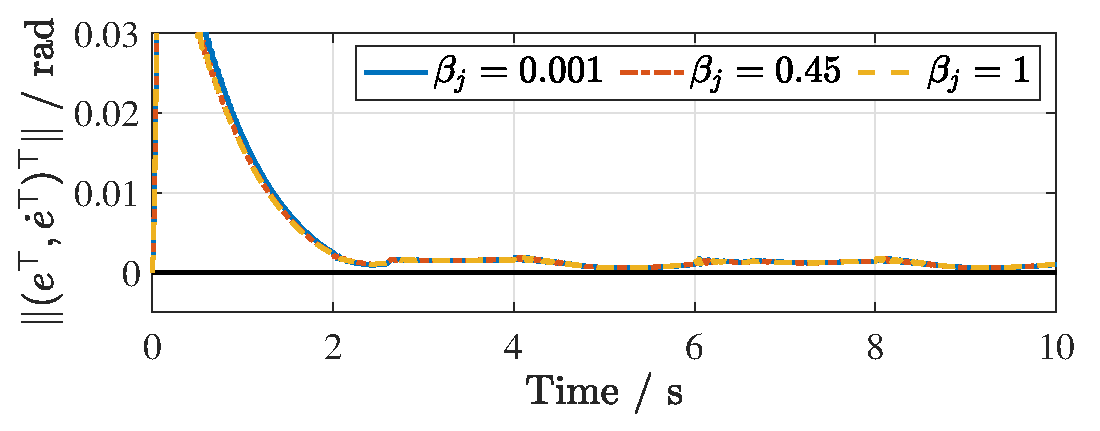
\includegraphics[width=0.99\textwidth]{figures/ECC/fig5.eps}
        \caption{Tracking error of NAC-CO}
      \end{figure}
    
  \end{columns}

  The Tracking error ...

\end{frame}

\section{Conclusion}

\subsection{Conclusion and Future Work}

\begin{frame}{Conclusion}
    
  Flux theme comes with three pre-defined block style collections.\\
  % Native style (default) available as \verb+\setblockstyle{native}+\\[0.5cm]
  
  \centering
	\begin{minipage}[b]{0.5\textwidth}

	  \begin{block}{Default}
        Block content.
      \end{block}

      \begin{alertblock}{Alert}
        Block content.
      \end{alertblock}

      \begin{exampleblock}{Example}
        Block content.
      \end{exampleblock}      
      
	\end{minipage}
\end{frame}

\section{}
\begin{frame}{}
    \centering \Large
    \emph{Thank you for your attention!}
\end{frame}

\begin{frame}[allowframebreaks]{References}

  \bibliography{../template/refs}
  \bibliographystyle{ieeetr}

\end{frame}

\end{document}